\chapter{Сессии}\label{chap:sessions}

HTTP является протоколом без состояния. И хотя некоторые рассматривают это как
недостаток, сторонники RESTful веб-разработки восхваляют это как плюс. Ведь
когда состояние отсутствует, мы автоматически получаем некоторые преимущества,
например, упрощение масштабируемости и кеширование.  В общем, вы можете
провести много параллелей с неизменяемой природой Haskell.

Насколько это возможно, RESTful приложениям следует избегать сохранения
состояния с информацией о взаимодействии с клиентом. Тем не менее, иногда это
неизбежно. Классическим примером является такая функциональность, как корзина
покупок, но и другие, более обычные взаимодействия, наподобие должной обработки
входа в систему, могут быть значительно улучшены путём правильного
использования сессий.

В этой главе описывается, как Yesod сохраняет данные сессии, как вы можете
получить доступ к этим данным, а также некоторые специальные функции, которые
помогут вам использовать сессии наилучшим образом.

\section{Clientsession}

Одним из первых пакетов, которые отделились от Yesod, был
\footnotehref{http://hackage.haskell.org/package/clientsession}{clientsession}.
Этот пакет использует шифрование и подписи для хранения данных в куки-файлах на
стороне клиента. Шифрование препятствует изучению данных пользователем, а
подпись гарантирует, что сессия не была ни захвачена, ни изменена.

Возможно, с точки зрения эффективности, хранение данных в куки звучит как
плохая идея. В конце концов, это означает, что данные должны отправляться с
каждым запросом. Однако на практике, clientsession может значительно улучшить
производительность.

\begin{itemize}
  \item Для обработки запроса не требуется обращаться к базе данных на стороне
      сервера.

  \item Легко масштабировать по горизонтали: каждый запрос содержит всю
      информацию, необходимую для ответа.

  \item Для того чтобы уменьшить нагрузку на канал, сайты могут предоставлять
      статический контент с отдельного доменного имени, таким образом избегая
      отправки куки сессии с каждым запросом.
\end{itemize}

Сохранение мегабайт информации в сессии будет плохой идеей. И поэтому
большинство рекомендаций по реализаций сессий не рекомендуют такую практику.
Если вам действительно нужно сберегать много данных для пользователя, то лучше
хранить ключ поиска в сессии, а фактические данные в базе данных.

Всё взаимодействия с clientsession обрабатывается внутри Yesod, но есть
несколько мест, где вы можете немного настроить его поведение.

\section{Управление сессией}
По умолчанию, ваше Yesod приложение будет использовать clientsession для
хранения данных сессии, получая ключ шифрования из
файла~\texttt{client-session-key.aes} и устанавливая для сессии двухчасовой
тайм-аут. (На замётку: тайм-аут измеряется с момента последнего запрос
пользователя к сайту, а \textbf{не} с момента создания сессии.) Однако, эти
установки могут быть изменены путём переопределения
метода~\lstinline'makeSessionBackend' класса типов~\lstinline'Yesod'.

Первый простой метод переопределения этого метода~--- просто отключить работу с
сессиями; для этого верните из метода~\lstinline'Nothing'. Если вашему
приложению абсолютно не требуются сессии, их отключение может дать небольшой
прирост производительности. Но будьте осторожны при отключении: оно также
отключит другие возможности, например, защиту от подделки кросс-сайтовых
запросов (Cross-Site Request Forgery, CSRF).

\begin{lstlisting}
    instance Yesod App where
        makeSessionBackend _ = return Nothing
\end{lstlisting}

Другой распространённый подход~--- изменить путь к файлу с ключом или значение
тайм-аута, но продолжить использование clientsession. В этом случае,
используйте вспомогательную функцию~\lstinline'defaultClientSessionBackend'.

\begin{lstlisting}
instance Yesod App where
    makeSessionBackend _ = do
        let minutes = 24 * 60 -- 1 day
            filepath = "mykey.aes"
        backend <- defaultClientSessionBackend minutes filepath
\end{lstlisting}

Есть ещё несколько функций, дающих точечное управление клиентскими сессиями, но
они редко требуются. Если заинтересовались, посмотрите документацию для
модуля~\lstinline'Yesod.Core'. Также возможна реализация других форм работы с
сессиями, например, сессии на стороне сервера. Насколько мне известно, на
момент написания таких реализаций нет.

\begin{remark}
    Если указанный файл с ключом не существует, он будет создан со
    сгенерированным случайным образом ключом. При развёртывании вашего
    приложения на боевую среду, вам следует включать заранее созданный ключ,
    иначе всё существующие сессии будут инвалидированы при создании нового
    файла с ключом. Это же верно и для случая использования каркаса сайта.
\end{remark}

\section{Работа с сессией}

Как и в большинстве фреймворков, сессия в Yesod представляет собой хранилище
пар ключ-значение. Базовое API сессии сводится к четырём функциям:
\lstinline'lookupSession' получает значение для ключа (если имеется),
\lstinline'getSession' возвращает всё пары ключ/значение,
\lstinline'setSession' задаёт значение для ключа, а \lstinline'deleteSession'
очищает значение для ключа.

\includecode{09/session-example.hs}

\section{Сообщения}

Одно из применений сессий~--- это сообщения. Они используются, чтобы решить
одну из обычных задач в веб-разработке: пользователь выполняет POST запрос,
веб-приложение делает изменения, а затем должно \emph{одновременно}
перенаправить пользователя на новую страницу и отправить ему сообщение об
успехе. (Это известно как Post/Redirect/Get).

Yesod предоставляет пару функций для реализации такого подхода:
\lstinline'setMessage' сохраняет значение в сессии, а \lstinline'getMessage'
одновременно считывает последнее значение в сессии и очищает старое значение,
чтобы оно не отобразилось дважды.

Рекомендуется вызывать \lstinline'getMessage' в \lstinline'defaultLayout',
чтобы любое доступное сообщение показывалось пользователю немедленно, без
необходимости помнить о добавлении вызова \lstinline'getMessage' в каждом
обработчике.

\includecode{09/messages.hs}

\begin{figure}[tbh]
  \centering
  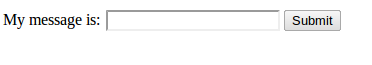
\includegraphics{09-sessions-image-01.png}
  \caption{Первая загрузка страницы, нет сообщения}
\end{figure}

\begin{figure}[tbh]
  \centering
  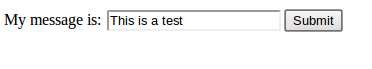
\includegraphics{09-sessions-image-02.png}
  \caption{Новое сообщение введено в текстовое поле}
\end{figure}

\begin{figure}[tbh]
  \centering
  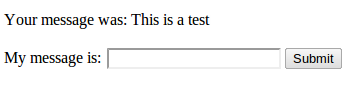
\includegraphics{09-sessions-image-03.png}
  \caption{После отправки формы, сообщение появляется в верхней части страницы}
\end{figure}

\begin{figure}[tbh]
  \centering
  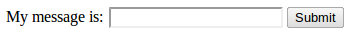
\includegraphics{09-sessions-image-04.png}
  \caption{После обновления, сообщение очищено}
\end{figure}

\section{Пункт назначения}

Не путайте с фильмом ужасов, пункт назначения~--- это техника, изначально
разработанная для фреймворка аутентификации Yesod, но имеющая более широкое
применение. Предположим, пользователь запрашивает страницу, которая требует
аутентификации. Если пользователь ещё не вошёл в систему, вам нужно отправить
его на страницу входа. Хорошо продуманное веб-приложение затем \emph{отправит
    его обратно на первоначально запрошенную страницу}. Это то, что мы называем
пунктом назначения.

Функция \lstinline'redirectUltDest' отправляет пользователя в пункт назначения,
установленный в его сессии, очищая это значение в сессии. Так же она берёт
значение по умолчанию, в случае, если значение пункта назначения не
установлено. Для установки сессии, есть три варианта:

\begin{itemize}
  \item \lstinline'setUltDest' устанавливает пункт назначения в данный URL,
      который может быть либо текстовым, либо типобезопасным URL.

  \item \lstinline'setUltDestCurrent' устанавливает пункт назначения в текущий
      запрошенный URL.

  \item \lstinline'setUltDestReferer' устанавливает пункт назначения на основе
      заголовка \lstinline'Referer' (страница, которая привела пользователя на
      текущую страницу).
\end{itemize}

Дополнительно есть функция \lstinline'clearUltDest' для удаления пункта
назначения из сессии, если он там присутствует.

Давайте рассмотрим небольшой пример приложения. Оно позволит пользователю
задать его имя в сессии, а затем скажет ему его имя с другого маршрута. Если
имя ещё не было установлено, пользователь будет перенаправлен на страницу ввода
имени, с пунктом назначения, установленным в возврат к текущей странице.

\includecode{09/ultimate-destination.hs}

\section{Выводы}

Сессии~--- это важнейшее средство, с помощью которого мы преодолеваем
отсутствие состояния в HTTP. Но мы не должны использовать этот аварийный люк
всякий раз, когда хотим: отсутствие состояний в веб-приложениях~--- это хорошее
свойство, и мы должны уважать его, когда это возможно. Тем не менее, есть
определённые случаи, когда важно сохранять некоторое состояние.

В Yesod очень простой API для работы с сессиями. Он предоставляет хранилище пар
ключ-значение, и несколько удобных функций для работы с ними для типичных
сценариев использования. При правильном использовании, с небольшой нагрузкой,
сессии должны быть скромной частью вашей веб-разработки.
